\chapter{Anlagenverzeichnis}

\section{Zeitplanung}
\begin{table}[h!]
    \centering
\begin{tabular}{|  >{\columncolor{gray!40}\centering\arraybackslash}m{0.5cm} | m{11cm} | >{\centering\arraybackslash}m{3cm} |}
  \hline
  \rowcolor{gray!40}
  Nr. & Aufgabe & Zeitansatz [h] \\
  \hline
  \rowcolor{gray!20}
  & Analyse & 3 \\
  \hline
  1 & IST-Analyse & 1 \\
  \hline
  2 & Nutzenanalyse & 1 \\
  \hline
  3 & Schutzbedarfsanalyse & 1 \\
  \hline
  \rowcolor{gray!20}
  & Planung & 3 \\
  \hline
  4 & Proof of Concept & 3 \\
  \hline
  \rowcolor{gray!20}
  & Realisierung & 11 \\
  \hline
  5 & Entra-SSPR-Konfiguration & 3 \\
  \hline
  6 & Anpassung des Bestellformulars & 2 \\
  \hline
  7 & Erstellung des Fulfillment Prozesses & 6 \\
  \hline
  \rowcolor{gray!20}
  & Produktivnahme & 12 \\
  \hline
  8 & Benutzerdoku erstellen & 3 \\
  \hline
  9 & Lifecycleprozesse & 3 \\
  \hline
  10 & Stageing & 6 \\
  \hline
  \rowcolor{gray!20}
  & Abschluss & 10 \\
  \hline
  11 & IST-SOLL-Vergleich & 1 \\
  \hline
  13 & Dokumentation erstellen & 9 \\
  \hline
  \rowcolor{gray!60}
   & Summe & 40 \\
  \hline
\end{tabular}
    \caption{Zeitplanung}
    \label{tab:Zeitplanung}
\end{table}



\begin{figure}[H]
\section{Projektlaufzeit}
    \centering
    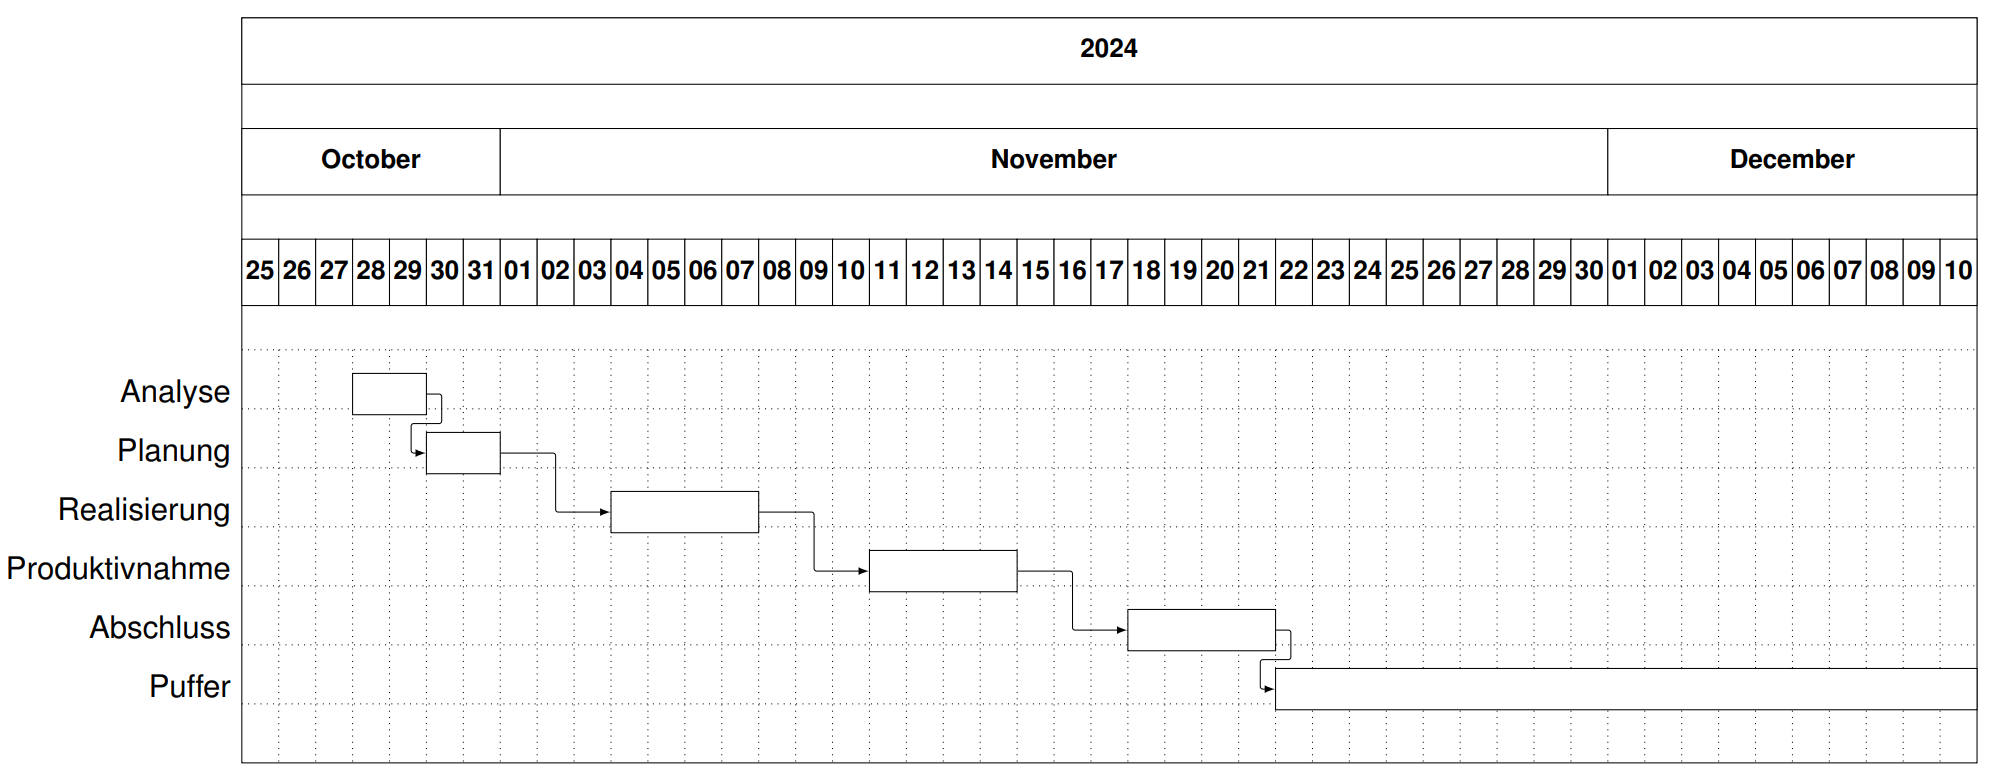
\includegraphics[width=1.0\textwidth]{Projektdokumentation/img/Projektlaufzeit.png}
    \caption{Projektlaufzeit}
    \label{fig:Projektlaufzeit}
\end{figure}

\section{Schutzbedarfsanalyse}
\begin{table}[H]
\centering
\begin{tabular}{|l|c|c|c|c|}
\hline
\textbf{ }          & \textbf{Vertraulichkeit} & \textbf{Integrität} & \textbf{Verfügbarkeit} & \textbf{Schutzbedarf gesamt} \\ \hline
MIM                         & Hoch                    & Mittel              & Hoch                   & Hoch                         \\ \hline
Verfügbarkeit der Daten     & Niedrig                 & Mittel              & Hoch                   & Mittel                       \\ \hline
\end{tabular}
\caption{Schutzbedarfsanalyse}
\label{tab:schutzbedarfsanalyse}
\end{table}

\begin{figure}[H]
\section{Authentifkationsmethoden}
    \centering
    
\includegraphics[width=1.0\textwidth]{Projektdokumentation/img/testing.jpg}
    \caption{Authentifkationsmethoden}
    \label{fig:Authentifkationsmethoden}
\end{figure}

\begin{figure}[H]
\section{SSPR-Gruppe}
    \centering
    
\includegraphics[width=1.0\textwidth]{Projektdokumentation/img/testing.jpg}
    \caption{SSPR-Gruppe}
    \label{fig:SSPR-Gruppe}
\end{figure}

\section{Bestellformular für einen externen Benutzer}
\begin{figure}[H]
    \centering
    
\includegraphics[width=1\textwidth]{Projektdokumentation/img/testing.jpg}
    \caption{Bestellformular}
    \label{fig:Bestellformular}
\end{figure}


\begin{figure}[H]
\section{Audit Logs}
    \centering
    
\includegraphics[width=1.0\textwidth]{Projektdokumentation/img/testing.jpg}
    \caption{Audit Logs}
    \label{fig:Audit Logs}
\end{figure}


\section{Vergleich Zeitplanung}

\begin{table}[H]
    \centering
\begin{tabular}{|  >{\columncolor{gray!40}\centering\arraybackslash}m{0.5cm} | m{6.5cm} | >{\centering\arraybackslash}m{3.5cm} | >{\centering\arraybackslash}m{3.5cm} |}
  \hline
  \rowcolor{gray!40}
  Nr. & Aufgabe & Zeitansatz [h] & Benötigt [h] \\
  \hline
  \rowcolor{gray!20}
  & Analyse & 3 &3\\
  \hline
  1 & IST-Analyse &\cellcolor{yellow!25} 1 &\cellcolor{yellow!25} 1 \\
  \hline
  2 & Nutzenanalyse &\cellcolor{yellow!25} 1 &\cellcolor{yellow!25} 1 \\
  \hline
  3 & Schutzbedarfsanalyse &\cellcolor{yellow!25} 1 &\cellcolor{yellow!25}1 \\
  \hline
  \rowcolor{gray!20}
  & Planung & 3 & 3\\
  \hline
  4 & Proof of Concept &\cellcolor{yellow!25} 3 &\cellcolor{yellow!25} 3 \\
  \hline
  \rowcolor{gray!20}
  & Realisierung & 11 & 11 \\
  \hline
  5 & Entra-SSPR-Konfiguration &\cellcolor{blue!25} 3 &\cellcolor{blue!25} 2 \\
  \hline
  6 & Anpassung des Bestellformulars &\cellcolor{blue!25} 2 &\cellcolor{blue!25} 4 \\
  \hline
  7 & Erstellung des Fulfillment Prozesses &\cellcolor{blue!25} 6 &\cellcolor{blue!25} 5 \\
  \hline
  \rowcolor{gray!20}
  & Produktivnahme & 12 & 12 \\
  \hline
  8 & Benutzerdoku erstellen &\cellcolor{yellow!25} 3 &\cellcolor{yellow!25} 3 \\
  \hline
  9 & Lifecycleprozesse &\cellcolor{yellow!25} 3 &\cellcolor{yellow!25} 3\\
  \hline
  10 & Staging &\cellcolor{yellow!25} 6 &\cellcolor{yellow!25} 6\\
  \hline
  \rowcolor{gray!20}
  & Abschluss & 10 & 10\\
  \hline
  11 & IST-SOLL-Vergleich &\cellcolor{blue!25} 1 &\cellcolor{blue!25} 2 \\
  \hline
  13 & Dokumentation erstellen &\cellcolor{blue!25} 9 &\cellcolor{blue!25} 8 \\
  \hline
  \rowcolor{gray!60}
   & Summe & 40 & 40\\
  \hline
\end{tabular}
    \caption{Vergleich Zeitplanung}
    \label{tab:Vergleich Zeitplanung}
\end{table}






